\large
	\def\imbcircle{(-210:2) circle (2.725cm)}
	\def\dscircle{(-330:2) circle (2.725cm)}
	\def\mdcircle{(-90:2) circle (2.725cm)}

	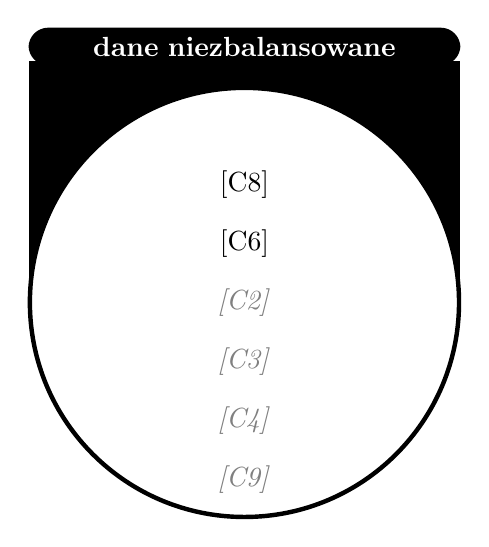
\begin{tikzpicture}
      	
      	\node[fill=black,rotate=0, text width=5.25cm, text height=2.9cm] at (90:-.5) {};
		\node[color=white,fill=black,rotate=0,rounded corners=.25cm, text width=5.25cm, align=center] at (90:1.25) {\bfseries \textsc{dane niezbalansowane}};
      	
      	\draw[fill=white] \mdcircle;
      	\draw[ultra thick] \mdcircle;
      	
      	\node at (-90:.5) {[C8]};    
      	\node at (-90:1.25) {[C6]};          	
      	    	   
      	\node at (-90:2) {\color{black!50}\emph{[C2]}};   
      	\node at (-90:2.75) {\color{black!50}\emph{[C3]}};   
      	\node at (-90:3.5) {\color{black!50}\emph{[C4]}};   
      	\node at (-90:4.25) {\color{black!50}\emph{[C9]}};
	\end{tikzpicture}